%!TEX TS-program = pdflatex
%!TEX encoding = windows-1250
\documentclass[a4paper, 12pt]{article}

\usepackage[utf8]{inputenc}
\usepackage{graphicx}

\usepackage{ifxetex}

\ifxetex
  \usepackage{fontspec}
  \usepackage{xltxtra}
  \usepackage[czech]{babel}
\else
  \usepackage[cp1250]{inputenc}
  \usepackage[czech]{babel}
\fi

\usepackage{bakalarska_prace}

\begin{document}

%
% souhrn
%
\section*{Souhrn}

Souhrn v ČJ

\section*{Summary}
Souhrn v AJ

%
% podekovani
%
\newpage
\section*{Poděkování}
případné poděkování. Pokud není, stranu vynechat.
\newpage
\tableofcontents
\newpage

\section{Úvod}
Toto je první kapitola.

\newpage
\section{Programování v Pythonu - historie a současnost}

\subsection{Vznik programovacího jazyka Python}
Prvni kapitola \ldots .

\subsection{Specifika programování v Pythonu}
Druha kapitola \ldots .

\subsection{Tvorba uživatelského rozhraní v Pythonu}
Treti kapitola \ldots .

\subsubsection{Obecné}
Možnosti tvorby UI v Pythonu \ldots .
\subsubsection{PyQt vs. Tkinter}
Porovnání použitého a nejčastěji používaného frameworku. \ldots .


\subsection{Technické pokyny k~vypracování bakalářské práce}
\subsubsection*{Forma psaní}
Text práce pište písmem s~patkou (Times) o velikosti 11~nebo 12 b po jedné straně bílého hladkého papíru formátu A4. Šíři levého okraje nastavte na 3,5~cm, pravý, horní a dolní okraj minimálně 2 cm. Text musí být pouze v~jediném sloupci zarovnaném na obou stranách nebo jen vlevo. Stránky číslujte. Žádoucí je dodržování typografických pravidel: po větné čárce a~tečce musí být vždy mezera, text uvnitř závorek pokračuje bez mezery. Základní typografická pravidla jsou např. uvedena na adrese http://www.typo.cz .

\subsubsection*{Chemické vzorce a rovnice}
Chemické vzorce a rovnice můžeme psát v prostředí \texttt{mhchem} -- například \texttt{\textbackslash{}ce\{H2SO4\}} produkuje \ce{H2SO4}.

\subsubsection*{Matematické vztahy}
Píšeme zásadně v matematickém prostředí:
$$ a^2 + b^2 = c^2 $$

\subsubsection*{Tabulky}
\begin{table}[h]
\caption{Toto je název tabulky}
\begin{center}
\begin{tabular}{|l|l|}
\hline
1 & 2\\
\hline
3 & 4 a tato buňka pokračuje a pokračuje a pokračuje \\
5 & 6 \\
\hline
\end{tabular}
\end{center}
\end{table}

Nad každou tabulkou je uvedena arabská číslice jako pořadí tabulky a název, který vystihuje vzájemné vztahy uvedených veličin a také definuje společné podmínky, za kterých byly údaje pořízeny. Tabulky musí být přehledné, jasně a logicky uspořádané. Je vhodné je uvést všude tam, kde zajistí účinnější prezentaci údajů. Mimo nadpis může mít tabulka vysvětlivky týkající se souboru či jen jednotlivých parametrů, resp. hodnot. Ty se uvádějí pod tabulkou a označují se malým písmenem v podobě indexu.

\subsubsection*{Obrázky}
Pod každým obrázkem je arabská číslice jako pořadí obrázku a~legenda, která jej činí jednoznačně srozumitelným (tj. bez nutnosti hledat nezbytné informace v textu). Vlastní legenda se skládá z~výstižného popisu uvedených závislostí, významu použitých symbolů a podmínek, za jakých byly údaje získány.
Grafy slouží k zobrazení závislostí sledovaných veličin, nikoliv k~přesnému odečítání číselných hodnot. Proto je zbytečné uvádět na osách husté kótování a početné číselné značení. Obvykle postačí na osách 5~kót a 3~číselné hodnoty. Výjimku tvoří nomogramy, ve kterých je možné použít sítě. 
Grafy musí mít označené osy příslušnými symboly veličin, oddělenými čárkou od jejich rozměrů. Zlomek se vždy převádí na součin s dělitelem v~záporné mocnině 
(např. $kmol\,l^{-1} min^{-1}$). 
Při větším počtu grafů je nutné dodržet jednotný rozměr a vzhled (stejnou výšku a sílu popisu, sílu čar, kót apod.). Nevhodné je do obrázků vpisovat text (např. reakční podmínky, za kterých byla závislost získána), vysvětlení experimentálních bodů, strukturní vzorce či číselné údaje. Ty patří do legendy k obrázku. 
Pokud jsou v~práci převzaté obrázky např. z~anglických literárních zdrojů (obvykle skenované), je nutné nahradit všechny cizojazyčné popisky českými. Viz obr. č. \ref{fig:plocha} 

\begin{figure}
\centering
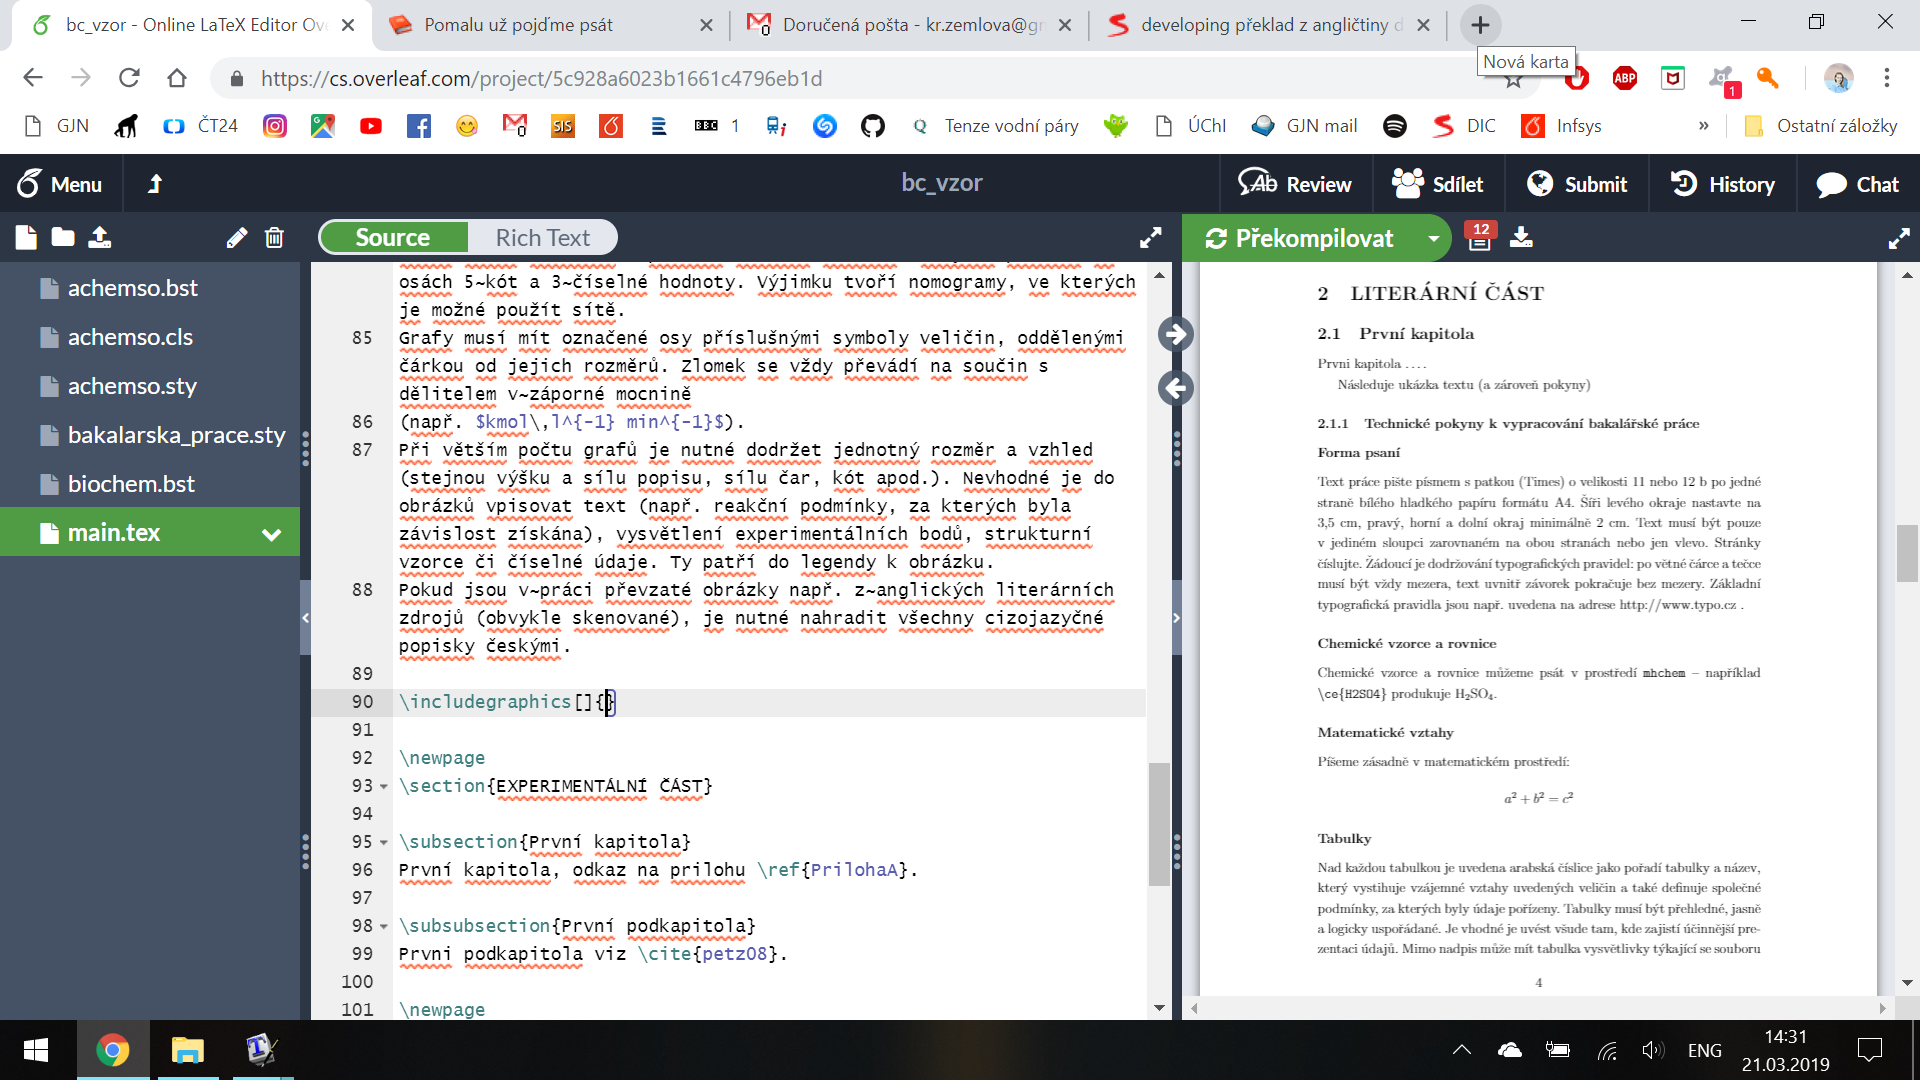
\includegraphics[width=15cm]{test.png}
\caption{Printscreen}
\label{fig:plocha}
\end{figure}

\newpage
\section{Zpracování signálu}
blabla úvod \ldots .

\subsection{Filtr s nulovým posunem}
\ldots .
\subsection{Savitzky-Golay filtr}
\ldots .
\subsection{Mediánový filtr}
\ldots .
\subsection{Exponenciální vyhlazování}
\ldots .

\newpage
\section{Tvorba uživatelského rozhraní a zpracování krystalografických dat}

\subsection{Hlavní okno a funkce}
\ref{PrilohaA}.
\subsubsection{Import dat a jejich vizualizace}
\cite{petz08}.
\subsubsection{Práce s daty, výběr kanálu}
\ldots .
\subsubsection{Záložky a funkce}
\ldots .

\subsection{Filtrace signálu}

\subsection{Export dat}
\ldots .

\newpage
\section{Výsledky a diskuse}

\newpage
\section{Závěr}


%%% Vytvoření seznamu literatury.
\newpage
\addcontentsline{toc}{section}{LITERATURA}

\bibliography{papers,books} % pozor, nesmi byt mezera


%%% Přílohy.
\newpage

\appendix

\section{Nějaké jméno přílohy}
\label{PrilohaA}


\end{document}
